% This LaTeX document needs to be compiled with XeLaTeX.
\documentclass[10pt]{article}
\usepackage[a4paper, margin=0.8in]{geometry}
\usepackage[utf8]{inputenc}
\usepackage{amsmath}
\usepackage{amsfonts}
\usepackage{amssymb}
\usepackage[version=4]{mhchem}
\usepackage{stmaryrd}
\usepackage{graphicx}
\usepackage[export]{adjustbox}
\graphicspath{ {./images/} }
\usepackage[fallback]{xeCJK}
\usepackage{polyglossia}
\usepackage{fontspec}
\usepackage{setspace}
\usepackage{enumitem}

\newcommand{\sol}{\textbf{解:} }

\onehalfspacing

\allowdisplaybreaks
\setcounter{section}{5}
\setcounter{subsection}{1}
\begin{document}
\subsection{圆的标准方程式}
\subsection*{(选择题)}

\begin{enumerate}[leftmargin=*]
  \item 求以 $(6,7)$ 与 $(4,-3)$ 之连线为直径之圆的方程式。

        \sol{}

        半径为 $\dfrac{\sqrt{(6-4)^{2}+(7-(-3))^{2}}}{2}=\dfrac{\sqrt{2^{2}+10^{2}}}{2}=\dfrac{\sqrt{104}}{2}=\dfrac{2\sqrt{26}}{2}=\sqrt{26}$,

        圆心为 $\left(\dfrac{6+4}{2}, \dfrac{7+(-3)}{2}\right)=(5,2)$, 所以方程式为 $(x-5)^{2}+(y-2)^{2}=26$。\hfill$\blacksquare$

  \item 如果圆 $x^{2}+y^{2}=4^{2}$ 上的一点 $P$ 到直线 $4 x+3 y-60=0$ 的距离是最小, 求 $P$ 点的坐标。

        \sol{}
        \begin{flalign*}
          4x + 3y - 60 & = 0                   \\
          3y           & = -4x + 60            \\
          y            & = -\dfrac{4}{3}x + 20 \\
          m            & = -\dfrac{4}{3}
        \end{flalign*}
        直线穿过圆心的法线方程为
        \begin{flalign*}
          y-0 & = \dfrac{3}{4}(x-0) \\
          y   & = \dfrac{3}{4}x
        \end{flalign*}
        代入圆的方程得
        \begin{flalign*}
          x^{2} + \left(\dfrac{3}{4}x\right)^{2} & = 4^{2}             \\
          x^{2} + \dfrac{9}{16}x^{2}             & = 16                \\
          \dfrac{25}{16}x^{2}                    & = 16                \\
          x^2                                    & = \dfrac{256}{25}   \\
          x                                      & = \pm \dfrac{16}{5}
        \end{flalign*}
        当 $x = \dfrac{16}{5}$ 时, $y = \dfrac{12}{5}$, 当 $x = -\dfrac{16}{5}$ 时, $y = -\dfrac{12}{5}$。\hfill$\blacksquare$

        所以 $P$ 点的坐标为 $\left(\dfrac{16}{5}, \dfrac{12}{5}\right)$。

  \item 求由圆 $(x-5)^{2}+(y-3)^{2}=9$ 上的一点到直线 $3 x+4 y=2$ 的最短距离。

        \sol{}

        直线 $3x+4y=2$ 与圆心 $(5,3)$ 的距离为 $\dfrac{|3(5)+4(3)-2|}{\sqrt{3^{2}+4^{2}}} = \dfrac{|15+12-2|}{5} = 5$。

        圆的半径为 $3$, 所以最短距离为 $5-3=2$。\hfill$\blacksquare$

        \newpage
  \item 点 $(5,3)$ 是圆 $(x-2)^{2}+(y+1)^{2}=25$ 的一直径的端点。求此直径另一端点的坐标。

        \sol{}

        设另一端点为 $(x, y)$, 已知圆心为 $(2, -1)$, 根据中点公式得
        \begin{flalign*}
          \dfrac{5+x}{2} & = 2  \\
          5+x            & = 4  \\
          x              & = -1 \\
          \dfrac{3+y}{2} & = -1 \\
          3+y            & = -2 \\
          y              & = -5
        \end{flalign*}
        所以另一端点的坐标为 $(-1, -5)$。\hfill$\blacksquare$
\end{enumerate}

\section*{(作答题)}
\begin{enumerate}[leftmargin=*]
  \item 一正方形的四顶点 $A, B, C, D$ 顺序依反时针方向排列。若 $A$ 点的座标为 $(1,3), BD$落于直线 $2 x+y+5=0$ 上。试求出 $B, C, D$ 三点的坐标。(不准用图解法。)

        \sol{}

        直线 $2x+y+5=0$ 的斜率为 $-2$, 该直线过点 $(1,3)$ 的法线斜率为 $\dfrac{1}{2}$, 所以法线方程为
        \begin{flalign*}
          y-3 & = \dfrac{1}{2}(x-1)                \\
          y   & = \dfrac{1}{2}x - \dfrac{1}{2} + 3 \\
          y   & = \dfrac{1}{2}x + \dfrac{5}{2}
        \end{flalign*}
        代入直线方程得
        \begin{flalign*}
          2x + \dfrac{1}{2}x + \dfrac{5}{2} + 5 & = 0                                   \\
          4x + x + 5 + 10                       & = 0                                   \\
          x                                     & = -3                                  \\
          y                                     & = \dfrac{1}{2}(-3) + \dfrac{5}{2} = 1
        \end{flalign*}
        所以正方形的中心为 $M(-3, 1)$。

        设 $B$ 点和 $C$ 点的坐标为 $(x, -2x-5)$。
        \begin{align*}
          \dfrac{AM}{MB}                                                    & = \tan 45^{\circ} = 1       \\
          \dfrac{\sqrt{(-3-1)^2 + (1 - 3)^2}}{\sqrt{(x+3)^2 + (-2x - 6)^2}} & = 1                         \\
          \sqrt{20}                                                         & = \sqrt{(x+3)^2 + 4(x+3)^2} \\
          20                                                                & = 5(x+3)^2                  \\
          4                                                                 & = (x+3)^2                   \\
          x + 3                                                             & = \pm 2                     \\
          x                                                                 & = -5, -1
        \end{align*}
        所以 $B$及 $D$ 的坐标分别为 $(-5, 5)$ 和 $(-1, -3)$。 \hfill$\blacksquare$

        设 $C$ 点的坐标为 $(x, y)$, 由正方形的性质得
        \begin{align*}
          \dfrac{x + 1}{2} & = -3 \\
          x                & = -7 \\
          \dfrac{y + 3}{2} & = 1  \\
          y                & = -1
        \end{align*}
        所以 $C$ 点的坐标为 $(-7, -1)$。\hfill$\blacksquare$

  \item 试求以 $A(2,0)$ 及 $B(6,0)$ 之联线为直径的圆之方程式。

        \sol{}

        圆心为 $\left(\dfrac{2+6}{2}, \dfrac{0+0}{2}\right) = (4, 0)$, 半径为 $\dfrac{\sqrt{(6-2)^{2}+(0-0)^{2}}}{2} = \dfrac{\sqrt{16}}{2} = 2$。

        所以方程式为
        \begin{flalign*}
          (x-4)^{2}+(y-0)^{2} & = 2^{2} \\
          (x-4)^{2}+y^{2}     & = 4     \\
          x^{2}-8x+16+y^{2}   & = 4     \\
          x^{2}-8x+y^{2}+12   & = 0
        \end{flalign*}\hfill$\blacksquare$

        若此圆与直线 $y=m x$ 相交于 $P$ 及 $Q$ 两点, 试证 $-\frac{1}{\sqrt{3}}<m<\frac{1}{\sqrt{3}}$ 。

        \sol{}
        \begin{align*}
          x^{2}-8 x+(m x)^{2}+12  & = 0 \\
          x^{2}-8 x+m^{2}x^{2}+12 & = 0 \\
          (1+m^{2})x^{2}-8x+12    & = 0 \\
          d = 8^{2}-4(1+m^{2})12 > 0    \\
          64-48(1+m^{2})> 0             \\
          48(1+m^{2}) < 64              \\
          1+m^{2} < \dfrac{4}{3}        \\
          m^{2} < \dfrac{1}{3}          \\
          -\dfrac{1}{\sqrt{3}} < m < \dfrac{1}{\sqrt{3}}
        \end{align*} \hfill$\blacksquare$

        又, 试求 $OP \times OQ$ 之值, 其中 $O$ 为原点。

        \sol{}

        设 $m = 0$, 则 $P(2, 0)$, $Q(6, 0)$, 所以 $OP \times OQ = 2 \times 6 = 12$。\hfill$\blacksquare$

        \newpage
  \item 已知两条直线 $l_{1}: 2 x-3 y+2=0$ 和 $l_{2}: 3 x-2 y+3=0$ 与圆心为 $M$ 的一圆相交, 且 $l_{1}$ 与 $l_{2}$ 被截在圆内的两条线段的长度分别为 26 及 24 , 求圆心 $M$ 的轨迹方程式。

        \sol{}

        设圆心为 $(x, y)$, 半径为 $r$,

        圆心到直线 $l_{1}$ 的距离为 $\dfrac{|2x-3y+2|}{\sqrt{2^{2}+(-3)^{2}}} = \dfrac{|2x-3y+2|}{\sqrt{13}}$,

        圆心到直线 $l_{2}$ 的距离为 $\dfrac{|3x-2y+3|}{\sqrt{3^{2}+(-2)^{2}}} = \dfrac{|3x-2y+3|}{\sqrt{13}}$。

        利用毕氏定理,得
        \begin{align*}
          r^{2} & = \left(\dfrac{|2x-3y+2|}{\sqrt{13}}\right)^{2} + 13^{2} \\
          r^2   & = \left(\dfrac{|3x-2y+3|}{\sqrt{13}}\right)^{2} + 12^{2}
        \end{align*}
        两式相等,
        \begin{align*}
          \left(\dfrac{|2x-3y+2|}{\sqrt{13}}\right)^{2} + 13^{2}                           & = \left(\dfrac{|3x-2y+3|}{\sqrt{13}}\right)^{2} + 12^{2} \\
          \dfrac{(2x-3y+2)^{2}}{13} + 169                                                  & = \dfrac{(3x-2y+3)^{2}}{13} + 144                        \\
          \dfrac{(2x-3y+2)^{2}}{13} - \dfrac{(3x-2y+3)^{2}}{13}                            & = -25                                                    \\
          (2x-3y+2)^{2} - (3x-2y+3)^{2}                                                    & = -325                                                   \\
          4x^{2} + 9y^{2} + 4 - 12xy - 12y + 8x - (9x^{2} + 4y^{2} + 9 - 12xy - 12y + 18x) & = -325                                                   \\
          4x^{2} + 9y^{2} + 4 - 12y + 8x - 9x^{2} - 4y^{2} - 9 + 12y - 18x                 & = -325                                                   \\
          -5x^{2} + 5y^{2} - 10x - 5                                                       & = -325                                                   \\
          5x^{2} - 5y^{2} + 10x - 320                                                      & = 0                                                      \\
          x^{2} - y^{2} + 2x - 64                                                          & = 0
        \end{align*} \hfill$\blacksquare$

  \item 已知 $A$ 点 $\left(x_{1}, y_{1}\right), B$ 点 $\left(x_{2}, y_{2}\right)$, 证明以 $AB$ 为直径的圆方程式为 $\left(x-x_{1}\right)\left(x-x_{2}\right)+\left(y-y_{1}\right)\left(y-y_{2}\right)=0$.

        一动圆经过一定点 $P(h, k)$ 与 $y$ 轴相切,求直径 $PR$ 的端点 $R$ 的轨迹方程式。

        \sol{}

        圆心为 $\left(\dfrac{x_{1}+x_{2}}{2}, \dfrac{y_{1}+y_{2}}{2}\right)$, 半径为 $\dfrac{\sqrt{(x_{2}-x_{1})^{2}+(y_{2}-y_{1})^{2}}}{2}$。

        所以圆的方程式为
        \begin{align*}
          \left(x-\dfrac{x_{1}+x_{2}}{2}\right)^{2} + \left(y-\dfrac{y_{1}+y_{2}}{2}\right)^{2}                                                   & = \left(\dfrac{\sqrt{(x_{2}-x_{1})^{2}+(y_{2}-y_{1})^{2}}}{2}\right)^{2}     \\
          x^2 - x(x_{1}+x_{2}) + \dfrac{x^{2}_{1}+2x_{1}x_{2}+x^{2}_{2}}{4} + y^{2} - y(y_{1}+y_{2}) + \dfrac{y^{2}_{1}+2y_{1}y_{2}+y^{2}_{2}}{4} & = \dfrac{x^{2}_{2}-2x_{1}x_{2}+x^{2}_{1}+y^{2}_{2}-2y_{1}y_{2}+y^{2}_{1}}{4} \\
          x^2 - x(x_{1}+x_{2}) + \dfrac{2x_{1}x_{2}}{4} + y^{2} - y(y_{1}+y_{2}) + \dfrac{2y_{1}y_{2}}{4}                                         & = \dfrac{-2x_{1}x_{2}-2y_{1}y_{2}}{4}                                        \\
          x^2 - x(x_{1}+x_{2}) + x_{1}x_{2} + y^{2} - y(y_{1}+y_{2}) + y_{1}y_{2}                                                                 & = 0                                                                          \\
          (x-x_{1})(x-x_{2}) + (y-y_{1})(y-y_{2})                                                                                                 & = 0
        \end{align*} \hfill$\blacksquare$

        设$R$点的坐标为 $(x, y)$, 半径为 $r$,则圆心为 $\left(\dfrac{h+x}{2}, \dfrac{k+y}{2}\right)$。
        \begin{align*}
          \left|\dfrac{h+x}{2}\right|                                           & = r                                        \\
          \left(x-\dfrac{h+x}{2}\right)^{2} + \left(y-\dfrac{k+y}{2}\right)^{2} & = r^{2}                                    \\
          \left(\dfrac{x-h}{2}\right)^{2} + \left(\dfrac{y-k}{2}\right)^{2}     & = r^{2}                                    \\
          \dfrac{(x-h)^{2}}{4} + \dfrac{(y-k)^{2}}{4}                           & = r^{2}                                    \\
          (x-h)^{2} + (y-k)^{2}                                                 & = 4r^{2}                                   \\
          x^{2} - 2hx + h^{2} + y^{2} - 2ky + k^{2}                             & = 4\left(\dfrac{h+x}{2}\right)^{2}         \\
          x^{2} - 2hx + h^{2} + y^{2} - 2ky + k^{2}                             & = 4\left(\dfrac{h^{2}+2hx+x^{2}}{4}\right) \\
          x^{2} - 2hx + h^{2} + y^{2} - 2ky + k^{2}                             & = h^{2} + 2hx + x^{2}                      \\
          y^{2} - 2ky + k^{2}                                                   & = 4hx                                      \\
          (y-k)^{2}                                                             & = 4hx
        \end{align*} \hfill$\blacksquare$

\end{enumerate}

\subsection{圆的一般方程式}
\subsection*{(选择题)}

\begin{enumerate}[leftmargin=*]
  \item 一圆的中心为 $(2,3)$ 且过点 $(3,-2)$, 求该圆之方程式。

        \sol{}

        圆心到点 $(3, -2)$ 的距离为 $\sqrt{(3-2)^{2}+(-2-3)^{2}} = \sqrt{1+25} = \sqrt{26}$,即为半径。

        所以方程式为
        \begin{flalign*}
          (x-2)^{2}+(y-3)^{2}   & = 26 \\
          x^{2}-4x+4+y^{2}-6y+9 & = 26 \\
          x^{2}+y^{2}-4x-6y-13  & = 0
        \end{flalign*}\hfill$\blacksquare$

  \item 求圆 $x^{2}+y^{2}-4 x-10 y+4=0$ 之半径。

        \sol{}
        \begin{align*}
          r & = \sqrt{(-2)^{2}+(-5)^{2} - 4} \\
            & = \sqrt{4+25-4} = 5
        \end{align*} \hfill$\blacksquare$

  \item 求圆 $x^{2}+y^{2}-6 x-4 y+9=0$ 之面积。

        \sol{}
        \begin{align*}
          r & = \sqrt{(-3)^{2}+(-2)^{2}-9} = \sqrt{9+4-9} = 2 \\
          S & = \pi r^{2} = 4\pi
        \end{align*}

  \item 若 $A$ 及 $B$ 分别为圆 $x^{2}+y^{2}-6 y=0$ 及 $x^{2}+y^{2}-6 x=0$ 的圆心, 则直线 $AB$ 之方程式为

        \sol{}
        \begin{align*}
          x^2 + y^2 - 6y & = 0 \Rightarrow x^2 + (y-3)^2 = 9 \\
          x^2 + y^2 - 6x & = 0 \Rightarrow (x-3)^2 + y^2 = 9
        \end{align*}
        两圆的圆心分别为 $A(0, 3)$ 及 $B(3, 0)$, 所以直线 $AB$ 的斜率为 $\dfrac{0-3}{3-0} = -1$,方程式为
        \begin{align*}
          y-3 & = -1(x-0) \Rightarrow x+y = 3
        \end{align*} \hfill$\blacksquare$

  \item 由点 $A(6,6)$ 至圆 $x^{2}+y^{2}-6 x-4 y+4=0$ 之最短距离为

        \sol{}
        \begin{align*}
          x^2 + y^2 - 6x - 4y + 4 & = 0              \\
          x^2 - 6x + y^2 - 4y     & = -4             \\
          (x-3)^2 + (y-2)^2       & = -4 + 9 + 4 = 9 \\
          (x-3)^2 + (y-2)^2       & = 3^2
        \end{align*}
        圆心为 $(3, 2)$, 半径为 $3$。

        点 $(6, 6)$ 到圆心的距离为 $\sqrt{(6-3)^{2}+(6-2)^{2}} = \sqrt{9+16} = 5$。

        所以最短距离为 $5-3 = 2$。\hfill$\blacksquare$

  \item 求点 $(9,4)$ 到圆 $x^{2}+y^{2}-4 x-6 y-5=0$ 的最短距离。

        \sol{}
        \begin{align*}
          x^2 + y^2 - 4x - 6y - 5 & = 0              \\
          x^2 - 4x + y^2 - 6y     & = 5              \\
          (x-2)^2 + (y-3)^2       & = 5 + 4 + 9 = 18 \\
          (x-2)^2 + (y-3)^2       & = (3\sqrt{2})^2
        \end{align*}
        圆心为 $(2, 3)$, 半径为 $3\sqrt{2}$。

        点 $(9, 4)$ 到圆心的距离为 $\sqrt{(9-2)^{2}+(4-3)^{2}} = \sqrt{49+1} = \sqrt{50} = 5\sqrt{2}$。

        所以最短距离为 $5\sqrt{2} - 3\sqrt{2} = 2\sqrt{2}$。\hfill$\blacksquare$

  \item 两个圆 $x^{2}+y^{2}-4 x-2 y-20=0$ 及 $x^{2}+y^{2}-6 x=0$ 的关系是

        \sol{}
        \begin{align*}
          x^2 + y^2 - 4x - 2y - 20 & = 0               \\
          x^2 - 4x + y^2 - 2y      & = 20              \\
          (x-2)^2 + (y-1)^2        & = 20 + 4 + 1 = 25 \\
          (x-2)^2 + (y-1)^2        & = 5^2
        \end{align*}
        圆心为 $(2, 1)$, 半径为 $5$。

        \newpage
        \begin{align*}
          x^2 + y^2 - 6x & = 0   \\
          x^2 - 6x + y^2 & = 0   \\
          (x-3)^2 + y^2  & = 9   \\
          (x-3)^2 + y^2  & = 3^2
        \end{align*}
        圆心为 $(3, 0)$, 半径为 $3$。

        $\because$ 两圆的圆新距离为 $\sqrt{(3-2)^{2}+(0-1)^{2}} = \sqrt{1+1} = \sqrt{2} < 5-3 = 2$。

        $\therefore$ 一个圆在另一个圆内。\hfill$\blacksquare$

  \item 求圆心为 $(-3,0)$ 且将圆 $x^{2}+y^{2}+2 x-4 y+1=0$ 的圆周加以平分的圆的方程式。

        \sol{}
        \begin{flalign*}
          x^{2}+y^{2}+2 x-4 y+1 & = 0 \\
          (x+1)^{2}+(y-2)^{2}   & = 4
        \end{flalign*}
        圆心为 $(-1, 2)$, 半径为 $2$。

        所求圆的圆心和 $(-1, -2)$ 所成的线段的斜率为 $\dfrac{0-(-2)}{-3-(-1)} = \dfrac{2}{2} = 1$。

        其过点 $(-1, 2)$ 的法线斜率为 $-1$,所以方程式为
        \begin{flalign*}
          y-2 & = -1(x+1) \Rightarrow y  = -x+1
        \end{flalign*}
        代入圆的方程得
        \begin{flalign*}
          (x+1)^{2} + (-x+1-2)^{2} & = 4               \\
          x^2 + 2x - 1             & = 0               \\
          x                        & = -1 \pm \sqrt{2}
        \end{flalign*}
        当 $x = -1 + \sqrt{2}$ 时, $y = 2 - \sqrt{2}$。

        所以所求圆的半径为 $\sqrt{(-3-(-1+\sqrt{2}))^{2}+(0-(2-\sqrt{2}))^{2}} = 2\sqrt{3}$,方程式为
        \begin{flalign*}
          (x+3)^{2}+y^{2}    & = (2\sqrt{3})^{2} \\
          x^{2}+6x+9+y^{2}   & = 12              \\
          x^{2}+6x+y^{2} - 3 & = 0
        \end{flalign*}\hfill$\blacksquare$

  \item 如果圆 $x^{2}+y^{2}+D x+E y+F=0$ 与 $x$ 轴相切于原点, 下列哪项是对的?

        \sol{}

        与$x$轴切于原点,则圆心在$y$轴上,半径等于圆心到原点的距离。
        \begin{align*}
          x^2 + (y - a)^2       & = a^2 \\
          x^2 + y^2 - 2ay + a^2 & = a^2 \\
          x^2 + y^2 - 2ay       & = 0
        \end{align*}
        所以 $D = 0$,$E = -2a$,$F = 0$。\hfill$\blacksquare$

  \item 已知 $P$ 及 $Q$ 分别是点 $(3,-2)$ 和 $(-1,4)$ 。若 $PQ$ 是一圆的直径, 求此圆的方程式。

        \sol{}

        圆心为 $\left(\dfrac{3-1}{2}, \dfrac{-2+4}{2}\right) = (1, 1)$, 半径为 $\dfrac{\sqrt{(3+1)^{2}+(-2-4)^{2}}}{2} = \dfrac{\sqrt{16+36}}{2} = \dfrac{\sqrt{52}}{2} = \sqrt{13}$。

        所以方程式为
        \begin{flalign*}
          (x-1)^{2}+(y-1)^{2}   & = (\sqrt{13})^{2} \\
          x^{2}-2x+1+y^{2}-2y+1 & = 13              \\
          x^{2}-2x+y^{2}-2y-11  & = 0
        \end{flalign*}\hfill$\blacksquare$

  \item 一圆心在 $x$ 轴上的圆经过 $A(-1,1)$ 及 $B(1,3)$ 两点。求此圆的方程式。

        \sol{}

        设圆心为 $(x, 0)$,则
        \begin{align*}
          \sqrt{(x+1)^{2}+1} & = \sqrt{(x-1)^{2}+9} \\
          (x+1)^{2}+1        & = (x-1)^{2}+9        \\
          x^{2}+2x+1+1       & = x^{2}-2x+1+9       \\
          4x                 & = 8                  \\
          x                  & = 2
        \end{align*}
        所以圆心为 $(2, 0)$, 半径为 $\sqrt{(2+1)^{2}+1} = \sqrt{9+1} = \sqrt{10}$。

        所以方程式为
        \begin{flalign*}
          (x-2)^{2}+y^{2}    & = 10 \\
          x^{2}-4x+4+y^{2}   & = 10 \\
          x^{2}+y^{2}-4x - 6 & = 0
        \end{flalign*}\hfill$\blacksquare$
\end{enumerate}

\subsection*{(作答题)}
\begin{enumerate}[leftmargin=*]
  \item \begin{enumerate}
          \item 求圆 $x^{2}+y^{2}-4 x+8 y-5=0$ 的圆心与半径。

                \sol{}
                \begin{align*}
                  x^{2}+y^{2}-4 x+8 y-5 & = 0               \\
                  x^{2}-4x+y^{2}+8y     & = 5               \\
                  (x-2)^{2}+(y+4)^{2}   & = 5 + 4 + 16 = 25 \\
                  (x-2)^{2}+(y+4)^{2}   & = 5^{2}
                \end{align*}
                $\therefore$ 圆心为 $(2, -4)$, 半径为 $5$。\hfill$\blacksquare$

          \item 设 $O$ 为坐标之原点, 若直线 $O C$ 割此圆于 $P, Q$ 两点, 求 $OP$ 及 $OQ$ 之长度。(注: $C$ 为圆心)

                \sol{}
                \begin{align*}
                  m_{OC}           & = \dfrac{0 - (-4)}{0 - 2} = \dfrac{4}{-2} = -2 \\
                  OC \Rightarrow y & = -2x
                \end{align*}
                将 $y = -2x$ 代入圆的方程得
                \begin{align*}
                  (x-2)^{2} + (-2x+4)^{2}            & = 25                         \\
                  x^{2} - 4x + 4 + 4x^{2} - 16x + 16 & = 25                         \\
                  5x^{2} - 20x + 20                  & = 25                         \\
                  5x^{2} - 20x - 5                   & = 0                          \\
                  x^{2} - 4x - 1                     & = 0                          \\
                  x                                  & = \dfrac{4 \pm 2\sqrt{5}}{2} \\
                                                     & = 2 \pm \sqrt{5}
                \end{align*}
                当 $x = 2 + \sqrt{5}$ 时, $y = -2(2 + \sqrt{5}) = -4 - 2\sqrt{5}$。

                当 $x = 2 - \sqrt{5}$ 时, $y = -4 + 2\sqrt{5}$。

                \begin{align*}
                  OP & = \sqrt{(2 + \sqrt{5})^{2} + (-4 - 2\sqrt{5})^{2}} \\
                     & = \sqrt{4 + 4\sqrt{5} + 5 + 16 + 16\sqrt{5} + 20}  \\
                     & = \sqrt{45 + 20\sqrt{5}}                           \\
                     & = \sqrt{45 + 2\sqrt{500}}                          \\
                     & = \sqrt{25 + 20 + 2\sqrt{25 \times 20}}            \\
                     & = 5 + 2\sqrt{5}
                \end{align*} \hfill$\blacksquare$
                \begin{align*}
                  OQ & = \sqrt{(2 - \sqrt{5})^{2} + (-4 + 2\sqrt{5})^{2}} \\
                     & = \sqrt{4 - 4\sqrt{5} + 5 + 16 - 16\sqrt{5} + 20}  \\
                     & = \sqrt{45 - 20\sqrt{5}}                           \\
                     & = \sqrt{45 - 2\sqrt{500}}                          \\
                     & = \sqrt{25 + 20 - 2\sqrt{25 \times 20}}            \\
                     & = 5 - 2\sqrt{5}
                \end{align*} \hfill$\blacksquare$

          \item 求此圆与 $x$-轴交点之坐标。

                \sol{}

                当 $y = 0$ 时,
                \begin{align*}
                  (x-2)^{2} + 4^{2} & = 25              \\
                  (x-2)^{2}         & = 9               \\
                  x                 & = 2 \pm 3         \\
                  x = 5             & \text{ 或 } x = -1
                \end{align*}
                $\therefore$ 交点为 $(5, 0)$ 及 $(-1, 0)$。\hfill$\blacksquare$

        \end{enumerate}

        \newpage
  \item 一圆切 $x$ 轴于 $(4,0)$, 截 $y$ 轴于 $(0,6)$ 。试求此圆之方程式。

        \sol{}
        设圆心为 $(h, k)$, 半径为 $r$。
        \begin{align*}
          (h-4)^{2} + k^{2} & = r^{2} \\
          h^{2} + (k-6)^{2} & = r^{2}
        \end{align*}
        比较两式得
        \begin{align*}
          (h-4)^{2} + k^{2}       & = h^{2} + (k-6)^{2}        \\
          h^{2} - 8h + 16 + k^{2} & = h^{2} + k^{2} - 12k + 36 \\
          -8h + 16                & = -12k + 36                \\
          12k - 8h                & = 20                       \\
          3k - 2h                 & = 5
        \end{align*}
        $\because$ 圆切 $x$ 轴于 $(4, 0)$, 则 $h = 4$。

        代入得 $3k - 8 = 5$,$k = \dfrac{13}{3}$。

        $\therefore$ 圆心为 $\left(4, \dfrac{13}{3}\right)$, 半径为 $\sqrt{(4-4)^{2} + \left(0-\dfrac{13}{3}\right)^{2}} = \dfrac{13}{3}$。

        方程式为
        \begin{align*}
          (x-4)^{2} + \left(y-\dfrac{13}{3}\right)^{2}              & = \left(\dfrac{13}{3}\right)^{2} \\
          x^{2} - 8x + 16 + y^{2} - \dfrac{26}{3}y + \dfrac{169}{9} & = \dfrac{169}{9}                 \\
          x^{2} + y^{2} - 8x - \dfrac{26}{3}y + 16                  & = 0                              \\
          3x^{2} + 3y^{2} - 24x - 26y + 48                          & = 0
        \end{align*} \hfill$\blacksquare$

  \item 求圆心在 $x$ 轴上, 且经过二已知圆 $x^{2}+y^{2}-2 x-14 y+25=0, x^{2}+y^{2}+2 x-2 y-3=0$的交点的圆之方程式。

        \sol{}
        \begin{flalign*}
          x^{2}+y^{2}-2 x-14 y+25 & = 0             \\
          x^2 + y^2               & = 2x + 14y - 25 \\
          x^{2}+y^{2}+2 x-2 y-3=0                   \\
          x^2 + y^2               & = -2x + 2y + 3
        \end{flalign*}
        比较两式得
        \begin{align*}
          2x + 14y - 25 & = -2x + 2y + 3 \\
          4x + 12y      & = 28           \\
          x + 3y        & = 7            \\
          x             & = 7 - 3y
        \end{align*}
        代入已知圆的方程得
        \begin{align*}
          (7-3y)^{2} + y^{2}        & = 2(7-3y) + 14y - 25 \\
          49 - 42y + 9y^{2} + y^{2} & = 14 - 6y + 14y - 25 \\
          10y^{2} - 50y + 60        & = 0                  \\
          y^{2} - 5y + 6            & = 0                  \\
          (y-2)(y-3)                & = 0                  \\
          y                         & = 2 \text{ 或 } y = 3
        \end{align*}
        当 $y = 2$ 时, $x = 7 - 3 \times 2 = 1$; 当 $y = 3$ 时, $x = 7 - 3 \times 3 = -2$。

        $\therefore$ 两圆的交点为 $(1, 2)$ 及 $(-2, 3)$。

        $\because$ 圆心在 $x$ 轴上,所以圆心为 $(h, 0)$。
        \begin{align*}
          \sqrt{(h-1)^{2} + 2^{2}} & = \sqrt{(h+2)^{2} + 3^{2}} \\
          h^{2} - 2h + 1 + 4       & = h^{2} + 4h + 4 + 9       \\
          -6h + 5                  & = 13                       \\
          h                        & = -\dfrac{4}{3}
        \end{align*}
        $\therefore$ 圆心为 $\left(-\dfrac{8}{3}, 0\right)$,半径为 $\sqrt{\left(-\dfrac{4}{3}-1\right)^{2} + 2^{2}} = \sqrt{\dfrac{25}{9} + 4} = \dfrac{\sqrt{85}}{3}$。

        方程式为
        \begin{align*}
          \left(x+\dfrac{4}{3}\right)^{2} + y^{2}       & = \left(\dfrac{\sqrt{85}}{3}\right)^{2} \\
          x^{2} + \dfrac{8}{3}x + \dfrac{16}{9} + y^{2} & = \dfrac{85}{9}                         \\
          9x^{2} + 24x + 16 + 9y^{2}                    & = 85                                    \\
          9x^{2} + 9y^{2} + 24x - 69                    & = 0                                     \\
          3x^{2} + 3y^{2} + 8x - 23                     & = 0
        \end{align*} \hfill$\blacksquare$

  \item 求通过二圆 $x^{2}+y^{2}-2 y-7=0, x^{2}+y^{2}+4 x-5=0$ 的交点且圆心落于直线 $x+2 y+3=0$ 上的圆之方程式。

        \sol{}

        两圆的方程式相减得
        \begin{align*}
          4x + 2y + 2 & = 0 \Rightarrow 2x + y + 1 = 0 \Rightarrow y = -2x - 1
        \end{align*}
        代入圆的方程得
        \begin{align*}
          x^2 + (-2x-1)^2 + 4x - 5     & = 0                              \\
          x^2 + 4x^2 + 4x + 1 + 4x - 5 & = 0                              \\
          5x^2 + 8x - 4                & = 0                              \\
          (5x - 2)(x + 2)              & = 0                              \\
          x                            & = \dfrac{2}{5} \text{ 或 } x = -2
        \end{align*}

        当 $x = \dfrac{2}{5}$ 时, $y = -2 \times \dfrac{2}{5} - 1 = -\dfrac{9}{5}$。

        当 $x = -2$ 时, $y = -2 \times (-2) - 1 = 3$。

        $\therefore$ 两圆的交点为 $\left(\dfrac{2}{5}, -\dfrac{9}{5}\right)$ 及 $(-2, 3)$。

        \begin{align*}
          x + 2y + 3 & = 0 \Rightarrow x = -2y - 3
        \end{align*}
        设圆心为 $(-2y-3, y)$,半径为 $r$。
        \begin{align*}
          \sqrt{\left(-2y-3-\dfrac{2}{5}\right)^{2} + \left(y+\dfrac{9}{5}\right)^{2}}        & = \sqrt{\left(-2y-3+2\right)^{2} + (y-3)^{2}} \\
          \left(-2y-\dfrac{17}{5}\right)^{2} + \left(y+\dfrac{9}{5}\right)^{2}                & = (-2y-1)^{2} + (y-3)^{2}                     \\
          4y^{2} + \dfrac{68}{5}y + \dfrac{289}{25} + y^{2} + \dfrac{18}{5}y + \dfrac{81}{25} & = 4y^{2} + 4y + 1 + y^{2} + 9 - 6y            \\
          \dfrac{86}{5}y + \dfrac{74}{5}                                                      & = - 2y + 10                                   \\
          86y + 74                                                                            & = -10y + 50                                   \\
          96y                                                                                 & = -24                                         \\
          y                                                                                   & = -\dfrac{1}{4}                               \\
          x                                                                                   & = -2 \times -\dfrac{1}{4} - 3 = -\dfrac{5}{2}
        \end{align*}
        $\therefore$ 圆心为 $\left(-\dfrac{5}{2}, -\dfrac{1}{4}\right)$,半径为 $\sqrt{\left(-\dfrac{5}{2}-\dfrac{2}{5}\right)^{2} + \left(-\dfrac{1}{4}+\dfrac{9}{5}\right)^{2}} = \dfrac{\sqrt{173}}{4}$。

        方程式为
        \begin{align*}
          \left(x+\dfrac{5}{2}\right)^{2} + \left(y+\dfrac{1}{4}\right)^{2} & = \left(\dfrac{\sqrt{173}}{4}\right)^{2} \\
          x^{2} + 5x + \dfrac{25}{4} + y^{2} + \dfrac{y}{2} + \dfrac{1}{16} & = \dfrac{109}{16}                        \\
          16x^{2} + 90x + 100 + 16y^{2} + 8y + 1                            & = 173                                    \\
          16x^{2} + 16y^{2} + 80x + 8y - 72                                 & = 0                                      \\
          2x^{2} + 2y^{2} + 10x + y - 9                                     & = 0
        \end{align*} \hfill$\blacksquare$

  \item $C$ 为一圆, 其一弦之中点, 长度及方星式分别为 $(1,1), 8$ 及 $3 x-4 y+1=0$ 。若 $C$ 通过点 $(8,2)$, 求 $C$ 之方程式。

        \sol{}

        设弦与圆的交点为 $\left(x, \dfrac{3x+1}{4}\right)$,则
        \begin{align*}
          \sqrt{(x-1)^{2} + \left(\dfrac{3x+1}{4}-1\right)^{2}} & = 4                            \\
          (x-1)^{2} + \left(\dfrac{3x-3}{4}\right)^{2}          & = 16                           \\
          x^{2} - 2x + 1 + \dfrac{9x^{2}-18x+9}{16}             & = 16                           \\
          16x^{2} - 32x + 16 + 9x^{2} - 18x + 9                 & = 256                          \\
          25x^{2} - 50x + 25                                    & = 256                          \\
          25(x-1)^{2}                                           & = 256                          \\
          x-1                                                   & = \pm \dfrac{16}{5}            \\
          x                                                     & = 1 \pm \dfrac{16}{5}          \\
          x = \dfrac{21}{5}                                     & \text{ 或 }\ x = -\dfrac{11}{5}
        \end{align*}
        当 $x = \dfrac{21}{5}$ 时, $y = \dfrac{3 \times \dfrac{21}{5} + 1}{4} = \dfrac{17}{5}$。

        当 $x = -\dfrac{11}{5}$ 时, $y = \dfrac{3 \times \left(-\dfrac{11}{5}\right) + 1}{4} = -\dfrac{7}{5}$。

        所以已知$C$过点$(8, 2)$、$\left(\dfrac{21}{5}, \dfrac{17}{5}\right)$及$\left(-\dfrac{11}{5}, -\dfrac{7}{5}\right)$。

        设圆的方程式为 $x^{2} + y^{2} + 2gx + 2fy + c = 0$,代入三点得
        \begin{align*}
          68 + 16g + 4f + c                                    & = 0                \\
          16g + 4f + c                                         & = -68\ \cdots (1)  \\
          \dfrac{146}{5} + \dfrac{42g}{5} + \dfrac{34f}{5} + c & = 0                \\
          42g + 34f + 5c                                       & = -146\ \cdots (2) \\
          \dfrac{34}{5} - \dfrac{22g}{5} - \dfrac{14f}{5} + c  & = 0                \\
          22g + 14f - 5c                                       & = 34\ \cdots (3)
        \end{align*}
        \begin{align*}
          (3) + (2)     & \Rightarrow 64g + 48f = -112                    \\
                        & \Rightarrow 4g + 3f = -7 \ \cdots (4)           \\
          (1) \times 5  & \Rightarrow 80g + 20f + 5c = -340 \ \cdots (5)  \\
          (3) + (5)     & \Rightarrow 102g + 34f = -306                   \\
                        & \Rightarrow 3g + f = -9 \ \cdots (6)            \\
          (6) \times 3  & \Rightarrow 9g + 3f = -27 \ \cdots (7)          \\
          (4) - (7)     & \Rightarrow -5g = 20                            \\
                        & \Rightarrow g = -4                              \\
          \text{代入 }(6) & \Rightarrow 3 \times -4 + f = -9                \\
                        & \Rightarrow f = 3                               \\
          \text{代入 }(1) & \Rightarrow 16 \times -4 + 4 \times 3 + c = -68 \\
                        & \Rightarrow c = -16
        \end{align*}
        $\therefore$ 圆的方程式为 $x^{2} + y^{2} - 8x + 6y - 16 = 0$。\hfill$\blacksquare$

        \newpage
  \item 求通过点 $(1,-1)$ 和两圆 $x^{2}+y^{2}-4 x-2 y+2=0, x^{2}+y^{2}+3 x-1=0$ 的交点的圆的方程式。

        \sol{}

        题目有误 \hfill$\blacksquare$

  \item 试求通过两圆 $x^{2}+y^{2}-2 x+5 y-6=0$, $2 x^{2}+2 y^{2}+3 x-y+1=0$ 的交点且圆心在直线 $x+y=6$ 上的圆的方程式。

        \sol{}

        题目有误 \hfill$\blacksquare$


  \item 一圆的圆心为 $A(8,6)$, 并与另一圆 $5 x^{2}+5 y^{2}-32 x-24 y+75=0$ 内切, 求此圆的方程式。

        \sol{}
        \begin{align*}
          5 x^{2}+5 y^{2}-32 x-24 y+75 & = 0 \\
          x^{2}+y^{2}-6.4 x-4.8 y+15   & = 0
        \end{align*}
        内切圆圆心为 $(3.2, 2.4)$,半径为 $\sqrt{(-3.2)^2 + (-2.4)^2 - 15} = \sqrt{10.24 + 5.76 - 15} = \sqrt{1} = 1$。

        内切圆圆心至圆心的距离为 $\sqrt{(8-3.2)^2 + (6-2.4)^2} = \sqrt{4.8^2 + 3.6^2} = 6$。

        圆的半径为其圆心至内切圆的最长距离,即 $6 + 1 = 7$。

        $\therefore$ 圆的方程式为 $(x-8)^{2} + (y-6)^{2} = 49$。\hfill$\blacksquare$

  \item 两对直线对 $AB$ 与 $AD, CB$ 与 $CD$ 的方程式依序是

        $$
          \begin{aligned}
             & 2 x^{2}-5 x y+2 y^{2}-3 x-3 y-9=0 \\
             & 2 x^{2}-5 x y+2 y^{2}+3 x+3 y-9=0
          \end{aligned}
        $$

        \begin{enumerate}
          \item 求它们的交点 $A, B, C$ 与 $D$ 的坐标。

                \sol{}

          \item 试证四边形 $\mathrm{ABCD}$ 是一个菱形。

          \item 求此菱形的面积。
        \end{enumerate}

  \item 如图所示, 以 $A$ 为圆心之圆与直线 $y-6=0$ 及以 $B$ 为圆心之圆 $x^{2}+y^{2}-6 x+8 y=0$ 外切。求点 $A$ 的轨迹方程式。
        \begin{center}
          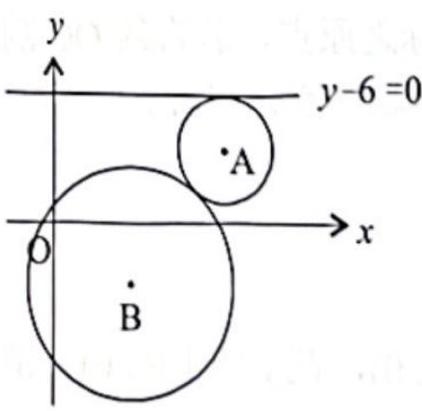
\includegraphics[max width=0.25\textwidth]{2024_06_07_f484519cd4dc635602b3g-04}
        \end{center}

  \item 已知 $A, B$ 两点的坐标分别是 $(-1,0)$ 及 $(0,2)$。若 $P$ 是圆 $x^{2}+y^{2}-2 x=0$ 上的任意点,求 $\triangle P A B$ 的面积的最大可能值。

\end{enumerate}

\newpage
\subsection{圆的切线}
\subsection*{(选择题)}

\begin{enumerate}[leftmargin=*]
  \item 求自 $x^{2}+y^{2}=50$, 在点 $(1,-7)$ 的切线方程式。

        \sol{}
        \begin{align*}
          x^{2}+y^{2}          & = 50            \\
          2x+2y \dfrac{dy}{dx} & = 0             \\
          \dfrac{dy}{dx}       & = -\dfrac{x}{y}
        \end{align*}
        当 $x = 1, y = -7$ 时, $\dfrac{dy}{dx} = -\dfrac{1}{-7} = \dfrac{1}{7}$。

        所以切线的斜率为 $\dfrac{1}{7}$,方程式为
        \begin{align*}
          y+7     & = \dfrac{1}{7}(x-1) \\
          7y + 49 & = x - 1             \\
          x - 7y  & = 50
        \end{align*} \hfill$\blacksquare$

  \item 求自点 $(3,3)$ 至圆 $x^{2}+y^{2}-2 x+4 y+1=0$ 的切线的长。

        \sol{}
        \begin{align*}
          x^{2}+y^{2}-2 x+4 y+1 & = 0                                                 \\
          \text{切距}             & = \sqrt{3^2 + 3^2 + (-2) \times 3 + 4 \times 3 + 1} \\
                                & = \sqrt{9 + 9 - 6 + 12 + 1}                         \\
                                & = \sqrt{25} = 5
        \end{align*} \hfill$\blacksquare$

  \item 求自点 $(3,4)$ 至圆 $x^{2}+4 x-4 y+4=0$ 的切线长。

        \sol{}
        \begin{align*}
          x^{2}+4 x-4 y+4 & = 0                                              \\
          \text{切距}       & = \sqrt{3^2 + 4^2 + 4 \times 3 - 4 \times 4 + 4} \\
                          & = \sqrt{9 + 16 + 12 - 16 + 4}                    \\
                          & = \sqrt{25} = 5
        \end{align*} \hfill$\blacksquare$

  \item 若直线 $2 x+3 y+3 \sqrt{13}=0$ 与圆 $x^{2}+y^{2}=k$ 相切, 则 $k$ 之值为

        \sol{}
        \begin{align*}
          2x + 3y + 3\sqrt{13} & = 0                          \\
          3y                   & = -2x - 3\sqrt{13}           \\
          y                    & = -\dfrac{2}{3}x - \sqrt{13} \\
          m_{\text{切线}}        & = -\dfrac{2}{3}
        \end{align*}
        \begin{align*}
          x^{2}+y^{2}           & = k             \\
          2x + 2y\dfrac{dy}{dx} & = 0             \\
          \dfrac{dy}{dx}        & = -\dfrac{x}{y} \\
          -\dfrac{2}{3}         & = -\dfrac{x}{y} \\
          y                     & = \dfrac{3}{2}x
        \end{align*}
        代入切线方程得
        \begin{align*}
          \dfrac{3}{2}x  & = -\dfrac{2}{3}x - \sqrt{13} \\
          \dfrac{13}{6}x & = -\sqrt{13}                 \\
          x              & = -\dfrac{6}{\sqrt{13}}      \\
          y              & = -\dfrac{9}{\sqrt{13}}
        \end{align*}
        $\therefore$ $k = \left(-\dfrac{6}{\sqrt{13}}\right)^{2} + \left(-\dfrac{9}{\sqrt{13}}\right)^{2} = \dfrac{36}{13} + \dfrac{81}{13} = \dfrac{117}{13} = 9$。\hfill$\blacksquare$

  \item 从点 $A(3,-4)$ 至圆 $x^{2}+y^{2}+6 x-8 y=0$ 所引切线, 其长等于

        \sol{}
        \begin{align*}
          x^{2}+y^{2}+6 x-8 y & = 0                                                    \\
          \text{切距}           & = \sqrt{3^{2} + (-4)^{2} + 6 \times 3 - 8 \times (-4)} \\
                              & = \sqrt{9 + 16 + 18 + 32}                              \\
                              & = \sqrt{75} = 5\sqrt{3}
        \end{align*} \hfill$\blacksquare$

  \item 若直线 $3 x-4 y=k$ 是圆 $x^{2}+y^{2}+2 x-4 y+1=0$ 的切线, 试求 $k$ 之值。

        \sol{}
        \begin{align*}
          x^{2}+y^{2}+2 x-4 y+1 & = 0          \\
          (x+1)^{2}+(y-2)^{2}   & = -1 + 4 + 1 \\
          (x+1)^{2}+(y-2)^{2}   & = 4
        \end{align*}
        圆心为 $(-1, 2)$, 半径为 $2$。
        \begin{align*}
          \left\vert \dfrac{3 \times (-1) - 4 \times 2 - k}{\sqrt{3^{2} + 4^{2}}} \right\vert & = 2           \\
          (11 + k)^2                                                                          & = 100         \\
          11 + k                                                                              & = \pm 10      \\
          k = -21                                                                             & \text{ 或 } -1
        \end{align*}

        \newpage
  \item 求从点 $(1,-2)$ 引圆 $(x-10)^{2}+(y-8)^{2}=15$ 的切线的长度。

        \sol{}
        \begin{align*}
          (x-10)^{2}+(y-8)^{2}       & = 15                                                           \\
          x^{2}-20x+100+y^{2}-16y+64 & = 15                                                           \\
          x^{2}+y^{2}-20x-16y+149    & = 0                                                            \\
          \text{切距}                  & = \sqrt{1^{2} + (-2)^{2} - 20 \times 1 - 16 \times (-2) + 149} \\
                                     & = \sqrt{1 + 4 - 20 + 32 + 149}                                 \\
                                     & = \sqrt{166}
        \end{align*}

  \item 求圆 $x^{2}+y^{2}=4$ 的切线的方程式, 它与圆的直径 $y=\frac{3}{4} x$ 平行。

        \sol{}
        $\because$ 切线与直径平行,所以切线的斜率为 $\dfrac{3}{4}$。
        \begin{align*}
          x^{2}+y^{2}          & = 4              \\
          2x+2y \dfrac{dy}{dx} & = 0              \\
          \dfrac{dy}{dx}       & = -\dfrac{x}{y}  \\
          -\dfrac{x}{y}        & = \dfrac{3}{4}   \\
          y                    & = -\dfrac{4}{3}x
        \end{align*}
        代入圆的方程得
        \begin{align*}
          x^{2} + \left(-\dfrac{4}{3}x\right)^{2} & = 4                \\
          x^{2} + \dfrac{16}{9}x^{2}              & = 4                \\
          \dfrac{25}{9}x^{2}                      & = 4                \\
          x^{2}                                   & = \dfrac{36}{25}   \\
          x                                       & = \pm \dfrac{6}{5}
        \end{align*}
        当 $x = \dfrac{6}{5}$ 时, $y = -\dfrac{4}{3} \times \dfrac{6}{5} = -\dfrac{8}{5}$。

        切线方程为
        \begin{align*}
          y + \dfrac{8}{5} & = \dfrac{3}{4}\left(x - \dfrac{6}{5}\right) \\
          y + \dfrac{8}{5} & = \dfrac{3}{4}x - \dfrac{9}{10}             \\
          y                & = \dfrac{3}{4}x - \dfrac{5}{2}
        \end{align*}

        \newpage
        当 $x = -\dfrac{6}{5}$ 时, $y = \dfrac{8}{5}$。

        切线方程为
        \begin{align*}
          y - \dfrac{8}{5} & = \dfrac{3}{4}\left(x + \dfrac{6}{5}\right) \\
          y - \dfrac{8}{5} & = \dfrac{3}{4}x + \dfrac{9}{10}             \\
          y                & = \dfrac{3}{4}x + \dfrac{5}{2}
        \end{align*}
        $\therefore$ 切线方程为 $y = \dfrac{3}{4}x \pm \dfrac{5}{2}$。\hfill$\blacksquare$

  \item 若直线 $y=-2 x+c$ 切圆 $x^{2}+y^{2}-6 x+12 y+40=0$, 则 $c$ 的值是

        \sol{}
        \begin{align*}
          y                                            & = -2x + c          \\
          m_{\text{切线}}                                & = -2               \\
          \\
          x^{2}+y^{2}-6x+12y+40                        & = 0                \\
          2x+2y \dfrac{dy}{dx} - 6 + 12 \dfrac{dy}{dx} & = 0                \\
          x + y \dfrac{dy}{dx} - 3 + 6 \dfrac{dy}{dx}  & = 0                \\
          (y+6) \dfrac{dy}{dx}                         & = 3 - x            \\
          \dfrac{dy}{dx}                               & = \dfrac{3-x}{y+6} \\
          -2                                           & = \dfrac{3-x}{y+6} \\
          x                                            & = 2y + 15
        \end{align*}
        代入圆的方程得
        \begin{align*}
          (2y + 15)^{2} + y^{2} - 6(2y + 15) + 12y + 40    & = 0                \\
          4y^{2} + 60y + 225 + y^{2} - 12y - 90 + 12y + 40 & = 0                \\
          y^{2} + 12y + 35                                 & = 0                \\
          (y+5)(y+7)                                       & = 0                \\
          y                                                & = -5 \text{ 或 } -7
        \end{align*}
        当 $y = -5$ 时, $x = 2 \times (-5) + 15 = 5$。
        \begin{align*}
          -5 & = -2 \times 5 + c \\
          c  & = 5
        \end{align*}
        当 $y = -7$ 时, $x = 2 \times (-7) + 15 = 1$。
        \begin{align*}
          -7 & = -2 \times 1 + c \\
          c  & = -5
        \end{align*}
        $\therefore$ $c = \pm 5$。\hfill$\blacksquare$

  \item 从点 $A(4, y)$ 向圆 $(x+3)^{2}+(y-4)^{2}=5^{2}$ 引切线, 则切距的最小值是

        \sol{}
        \begin{align*}
          (x+3)^{2}+(y-4)^{2}                 & = 25                                   \\
          x^{2} + 6x + 9 + y^{2} - 8y + 16    & = 25                                   \\
          x^{2} + y^{2} + 6x - 8y             & = 0                                    \\
          \text{切距}                           & = \sqrt{4^{2} + y^2 + 6 \times 4 - 8y} \\
                                              & = \sqrt{16 + y^2 + 24 - 8y}            \\
                                              & = \sqrt{40 + y^2 - 8y}                 \\
          \dfrac{d}{dy}(\sqrt{40 + y^2 - 8y}) & = 0                                    \\
          \dfrac{y - 4}{\sqrt{40 + y^2 - 8y}} & = 0                                    \\
          y                                   & = 4                                    \\
          \text{切距}                           & = \sqrt{40 + 4^2 - 8 \times 4}         \\
                                              & = \sqrt{40 + 16 - 32}                  \\
                                              & = \sqrt{24} = 2\sqrt{6}
        \end{align*}

  \item 如果直线 $y-2=k(x-1)$ 是圆 $x^{2}+y^{2}=1$ 的一条切线, 则此切线的方程式是

        \sol{}
        \begin{align*}
          y-2              & = k(x-1)     \\
          y                & = kx + 2 - k \\
          kx - y + (2 - k) & = 0
        \end{align*}
        圆心为 $(0, 0)$, 半径为 $1$。
        \begin{align*}
          \left\vert \dfrac{2-k}{\sqrt{1 + k^{2}}} \right\vert & = 1            \\
          (2-k)^{2}                                            & = 1 + k^{2}    \\
          4 - 4k + k^{2}                                       & = 1 + k^{2}    \\
          4k                                                   & = 3            \\
          k                                                    & = \dfrac{3}{4}
        \end{align*}
        $\therefore$
        \begin{align*}
          y - 2       & = \dfrac{3}{4}(x-1) \\
          4y - 8      & = 3x - 3            \\
          3x - 4y + 5 & = 0
        \end{align*}

        \newpage
  \item 两圆 $x^{2}+y^{2}+2 x-6 y-26=0$ 与 $x^{2}+y^{2}-4 x+2 y+4=0$ 有几条公切线?

        \sol{}
        两圆的方程式相减,得
        \begin{align*}
          6x - 8y - 30 & = 0                   \\
          3x - 4y - 15 & = 0                   \\
          y            & = \dfrac{3}{4}(x - 5)
        \end{align*}
        代入第一个圆的方程式得
        \begin{align*}
          x^{2} + \left(\dfrac{3}{4}(x - 5)\right)^{2} + 2x - 6 \times \dfrac{3}{4}(x - 5) - 26                   & = 0             \\
          x^{2} + \dfrac{9}{16}(x^{2} - 10x + 25) + 2x - \dfrac{9}{2}x + \dfrac{45}{2} - 26                       & = 0             \\
          x^{2} + \dfrac{9}{16}x^{2} - \dfrac{45}{8}x + \dfrac{225}{16} + 2x - \dfrac{9}{2}x + \dfrac{45}{2} - 26 & = 0             \\
          16x^{2} + 9x^{2} - 90x + 225 + 32x - 72x + 360 - 416                                                    & = 0             \\
          25x^{2} - 130x + 169                                                                                    & = 0             \\
          (5x - 13)^{2}                                                                                           & = 0             \\
          x                                                                                                       & = \dfrac{13}{5}
        \end{align*}
        $\because$ 两圆只有一个公共点,所以只有一条公切线。\hfill$\blacksquare$

  \item 直线 $7 x-24 y+8=0$ 是圆心为 $(2,3)$ 的圆的切线。求这个圆的半径。

        \sol{}
        \begin{align*}
          r & = \left\vert \dfrac{7 \times 2 - 24 \times 3 + 8}{\sqrt{7^{2} + 24^{2}}} \right\vert \\
            & = \left\vert \dfrac{14 - 72 + 8}{\sqrt{49 + 576}} \right\vert                        \\
            & = \left\vert \dfrac{-50}{\sqrt{625}} \right\vert                                     \\
            & = \left\vert \dfrac{-50}{25} \right\vert                                             \\
            & = 2
        \end{align*}

  \item 求圆 $x^{2}+y^{2}-6 x-4 y+4=0$ 上两条平行切线之间的距离。

        \sol{}
        \begin{align*}
          x^2 + y^2 - 6x - 4y + 4 & = 0          \\
          (x-3)^2 + (y-2)^2       & = -4 + 9 + 4 \\
          (x-3)^2 + (y-2)^2       & = 9
        \end{align*}
        $\therefore$ 圆心为 $(3, 2)$, 半径为 $3$。

        $\because$ 两条平行切线之间的距离为圆的直径

        $\therefore$ 两条平行切线之间的距离为 $2 \times 3 = 6$。

        \newpage
  \item 若从点 $(a, 1)$ 到圆 $x^{2}+y^{2}+5 x+7 y+3=0$ 的切线长是5 , 求 $a$ 的值。

        \sol{}
        \begin{align*}
          x^{2}+y^{2}+5 x+7 y+3                              & = 0               \\
          \text{切距}                                          & = 5               \\
          \sqrt{a^{2} + 1^{2} + 5 \times a + 7 \times 1 + 3} & = 5               \\
          \sqrt{a^{2} + 5a + 11}                             & = 5               \\
          a^{2} + 5a + 11                                    & = 25              \\
          a^{2} + 5a - 14                                    & = 0               \\
          (a + 7)(a - 2)                                     & = 0               \\
          a = -7                                             & \text{ 或 }\ a = 2
        \end{align*}
\end{enumerate}

% \section*{(作答题)}
% \begin{enumerate}[leftmargin=*]
%   \item 直线 $AB, AC$ 分别切圆 $O$ 于 $B, C$ 两点。求证 $AB=AC$ 。

%   \item 求切于 $x$ 轴及直线 $3 x-4 y+3=0$ 且约心在王线 $x+y=3$ 上的四之方罣式。

% \end{enumerate}

% [1978 年第 7 処]

% \begin{enumerate}[leftmargin=*]
%   \setcounter{enumi}{2}
%   \item 求自点 $P(4,2)$ 作因 $x^{2}+y^{2}-4 x+4 y-2=0$ 之切线的方䙵式。
% \end{enumerate}

% [1984 年第 3(a)题]

% \begin{enumerate}[leftmargin=*]
%   \setcounter{enumi}{3}
%   \item 求由一定点 $(2,2)$ 至圆 $2 x^{2}+2 y^{2}+2 x+4 y-1=0$ 的切距。
% \end{enumerate}

% [1987 年第 5(b)题]

% \begin{enumerate}[leftmargin=*]
%   \setcounter{enumi}{4}
%   \item 两圆都与 $x, y$ 两轴相切且通过点 $A(8,1)$ 。试求
% \end{enumerate}

% (i) 两圆的方程式:

% (ii) 两圆的另一交点之坐标;

% (iii) 在 $A$ 点每一圆的切线之方程式。

% (iv) 在 $A$ 点两切线所夹锐角。

% [1989 年第 6(a)题]

% \begin{enumerate}[leftmargin=*]
%   \setcounter{enumi}{5}
%   \item (a) 如果圆 $x^{2}+y^{2}+2 g x+2 f y+c=0$ 上一点 $\left(x_{0}, y_{0}\right)$ 所引切线与圆 $x^{2}+y^{2}=r^{2}$ 相切, 试证 $\left(g x_{0}+f y_{0}+c\right)^{2}=r^{2}\left(g^{2}+f^{2}-c\right)$ 。
% \end{enumerate}

% (b) 如果圆 $x^{2}+y^{2}-4 x-8 y-80=0$ 内的弦其长度及斜率分别为 $8 \sqrt{5}$ 及 $\frac{1}{2}$, 求这些弦的方程式。

% $[1990$ 年第 9 题]

% \begin{enumerate}[leftmargin=*]
%   \setcounter{enumi}{6}
%   \item 已知直线 $y=x+b$ 是圆 $x^{2}+y^{2}=4$ 的一条切线, 求 $b$ 的可能值。
% \end{enumerate}

% $[2000$ 年第 $7(b)$ 题 $]$

% \begin{enumerate}[leftmargin=*]
%   \setcounter{enumi}{7}
%   \item 在圆 $x^{2}+y^{2}=a^{2}$ 上一动点 $P$ 的切线分别交座标轴 $OX, OY$ 于 $A$ 和 $B$, 且 $\mathrm{OAQB}$ 是一个长方形。试证明 $Q$ 点的轨迹方程式是 $\frac{a^{2}}{x^{2}}+\frac{a^{2}}{y^{2}}=1$ 。
% \end{enumerate}

% [2002 年第 9 (c)题]

% \begin{enumerate}[leftmargin=*]
%   \setcounter{enumi}{8}
%   \item (a) 求经过圆 $x^{2}+y^{2}+2 x-4 y+1=0$ 与直线 $2 x-y+4=0$ 的交点且与 $y$ 轴相切的两圆的方程式。
% \end{enumerate}

% (b) 求过原点到此二圆所作的另两条切线的方程式。

% \begin{enumerate}[leftmargin=*]
%   \setcounter{enumi}{9}
%   \item 求 $x^{2}+y^{2}+4 x-10 y-7=0$ 的想心及半经。䁌此, 或其他方法, 若 $y=2 x+c$ 是此四的切线, 来 $c$ 的设。
% \end{enumerate}

% $(3 \%)$

% [2007 年第 7(a)廼]

% \begin{enumerate}[leftmargin=*]
%   \setcounter{enumi}{10}
%   \item 求两条由点 $(-2,3)$ 至目 $x^{2}+y^{2}+2 x-12 y+32=0$ 的切线方程式。
% \end{enumerate}

% [2010 年第 $7(b)$ 顷]

% \begin{enumerate}[leftmargin=*]
%   \setcounter{enumi}{11}
%   \item 求经过点 $M(3,-4)$ 且与圆 $x^{2}+y^{2}+2 x-6 y+5=0$ 相切于点 $P(1,2)$ 的圆的方程式。 $(6 \%)$ [2014 年第 $7(b)$ 輀 $]$
% \end{enumerate}

% \section*{[5.5] 两圆正切、正交}
% \section*{(选择题)}
% \begin{enumerate}[leftmargin=*]
%   \item 两圆 $x^{2}+y^{2}+3 x-2 y-20=0$ 及 $x^{2}+y^{2}-2 x+3 y-5=0$ 的公共弦的方程式是\\
% A $x+y-3=0$\\
% B $x-y-3=0$\\
% $x-y-5=0$\\
% D $2 x+y-3=0$\\
% E $\quad x-2 y+3=0$
% \end{enumerate}

% C

% [1987 年第 6 题]

% \begin{enumerate}[leftmargin=*]
%   \setcounter{enumi}{1}
%   \item 已知两圆 $x^{2}+y^{2}+k x-6 y+5=0$ 与 $x^{2}+y^{2}+2 x+y-1=0$ 正交(Cut orthogonally), $k$之值为\begin{enumerate}[leftmargin=*]。\\
% A -9\\
% B $\quad-7$\\
% C 5\\
% D 7\\
% E 9
% \end{enumerate}

% [1988 年第 19 题]

% \begin{enumerate}[leftmargin=*]
%   \setcounter{enumi}{2}
%   \item 如果两圆 $x^{2}+y^{2}=1$ 及 $x^{2}+y^{2}-6 x+a y+9=0$ 相切, 求 $a$ 的值。\\
% A $\pm 10$\\
% B $\pm 8$\\
% C $\pm 6$\\
% D $\pm 4$\\
% E 0
% \end{enumerate}

% [1992 年第 13 题]

% \begin{enumerate}[leftmargin=*]
%   \setcounter{enumi}{3}
%   \item 如果两圆 $x^{2}+y^{2}-4=0$ 及 $x^{2}+y^{2}+2 a x-6 y+a=0$ 正交(Cut orthogonally), 则常数 $a$的值等于\begin{enumerate}[leftmargin=*] -\\
% A 4\\
% B 3\\
% C 2\\
% D 1\\
% E 0
% \end{enumerate}

% [1992 年第 15 题]

% \begin{enumerate}[leftmargin=*]
%   \setcounter{enumi}{4}
%   \item 已知两圆 $(x-a)^{2}+(y-b)^{2}=c^{2}$ 与 $(x-b)^{2}+(y-a)^{2}=c^{2}$ 交于一点, 求 $a, b$ 及 $c$ 的关系。\\
% A $(a-b)^{2}=2 c^{2}$\\
% B $(a+b)^{2}=2 c^{2}$\\
% C $(a-b)^{2}=c^{2}$\\
% D $(a+b)^{2}=c^{2}$\\
% E 以上都不是

%   \item 若两圆 $x^{2}+y^{2}+6 x+10 y+c=0$ 与 $x^{2}+y^{2}+4 x-2 y+3=0$ 正交, 求 $c$ 的傎。\\
% A 3\\
% B 1\\
% C -1\\
% D $\quad-2$\\
% E -3

% \end{enumerate}

% [2012 年第 15 题]

% \begin{enumerate}[leftmargin=*]
%   \setcounter{enumi}{6}
%   \item 若两圆 $x^{2}+y^{2}-k x-2 y-52=0$ 与 $x^{2}+y^{2}+(2 k+1) x+8 y+26=0$ 正交, 求 $k$ 的值。\\
% A $-\frac{9}{2}$ 或 4\\
% B $-\frac{9}{2}$ 或 2\\
% C $\frac{9}{2}$ 或 -4\\
% D $\frac{9}{2}$ 或 -2\\
% E $\frac{9}{2}$ 或 2
% \end{enumerate}

% [2013 年第 15 题]

% \section*{(作答题)}
% \begin{enumerate}[leftmargin=*]
%   \item 二圆外切于 $A$, 公切线 $PQ$ 切二圆于 $P, Q ; RAS$ 是一直线且再遇二圆于 $R, S$, 连 $RP$, $S Q$ 并延长之使交于 $X$ 。求证
% \end{enumerate}

% (a) $\triangle APQ \sim \triangle XRS$;

% (b) $P, A, Q, X$ 四点共圆。

% [1976 年第 9 题]

% \begin{enumerate}[leftmargin=*]
%   \setcounter{enumi}{1}
%   \item 已知 $a^{2}+b^{2}=c^{2}$, 试证两圆 $x^{2}+y^{2}+a x+b y=0$ 及 $x^{2}+y^{2}=c^{2}$ 相切, 并求其切点之座标。

%   \item (a) 若两圆 $x^{2}+y^{2}+2 g_{1} x+2 f_{1} y+c_{1}=0$ 与 $x^{2}+y^{2}+2 g_{2} x+2 f_{2} y+c_{2}=0$ 正交, 证明

% \end{enumerate}

% $$
% 2\left(g_{1} g_{2}+f_{1} f_{2}\right)=c_{1}+c_{2}
% $$

% (b) 若一直径的两端点为 $(0,4)$ 及 $(4,2)$ 的圆与另一圆 $x^{2}+y^{2}+2 k x-6 y+k=0$ 正交, 试应用(a)的结果或以其他方法求 $k$ 的值。

% (3\%)

% [1996 年第 $8(b)(c)$ 题]

% \begin{enumerate}[leftmargin=*]
%   \setcounter{enumi}{3}
%   \item 一圆的圆心落在第一象限上且与 $y$ 轴相切于点 $(0,3)$, 并与圆 $x^{2}+y^{2}-8 x+4 y-5=0$ 正交。求此圆的方程式。
% \end{enumerate}

% [2004 年第 7(a)题]

% \begin{enumerate}[leftmargin=*]
%   \setcounter{enumi}{4}
%   \item 如果一个动圆与圆 $x^{2}+y^{2}+2 g x+2 f y+c=0$ 正交, 且与 $x$ 轴相切。求这个动圆圆心的轨迹方程式。

%   \item 已知两败的方侑式为 $x^{2}+y^{2}+2 x-6 y=0$ 及 $x^{2}+y^{2}+3 x-5 y+6=0$ 。 证明其中一完全在乐一婴内。

% \end{enumerate}

% $(40$

% [2011 年第 8(b) 勘

% \begin{enumerate}[leftmargin=*]
%   \setcounter{enumi}{6}
%   \item 已知一团 $C$ 的半径为 3. 其罒心在䛖械 $x+y=1$ 上。若圆 $x^{2}+y^{2}=4$ 内切于圆 $C, y$ C的所有可恠方㱐式。
% \end{enumerate}

% (4)

% [2012 年第 9(a) 题


\end{document}